\usetikzlibrary{positioning, arrows.meta, shapes.geometric, calc}
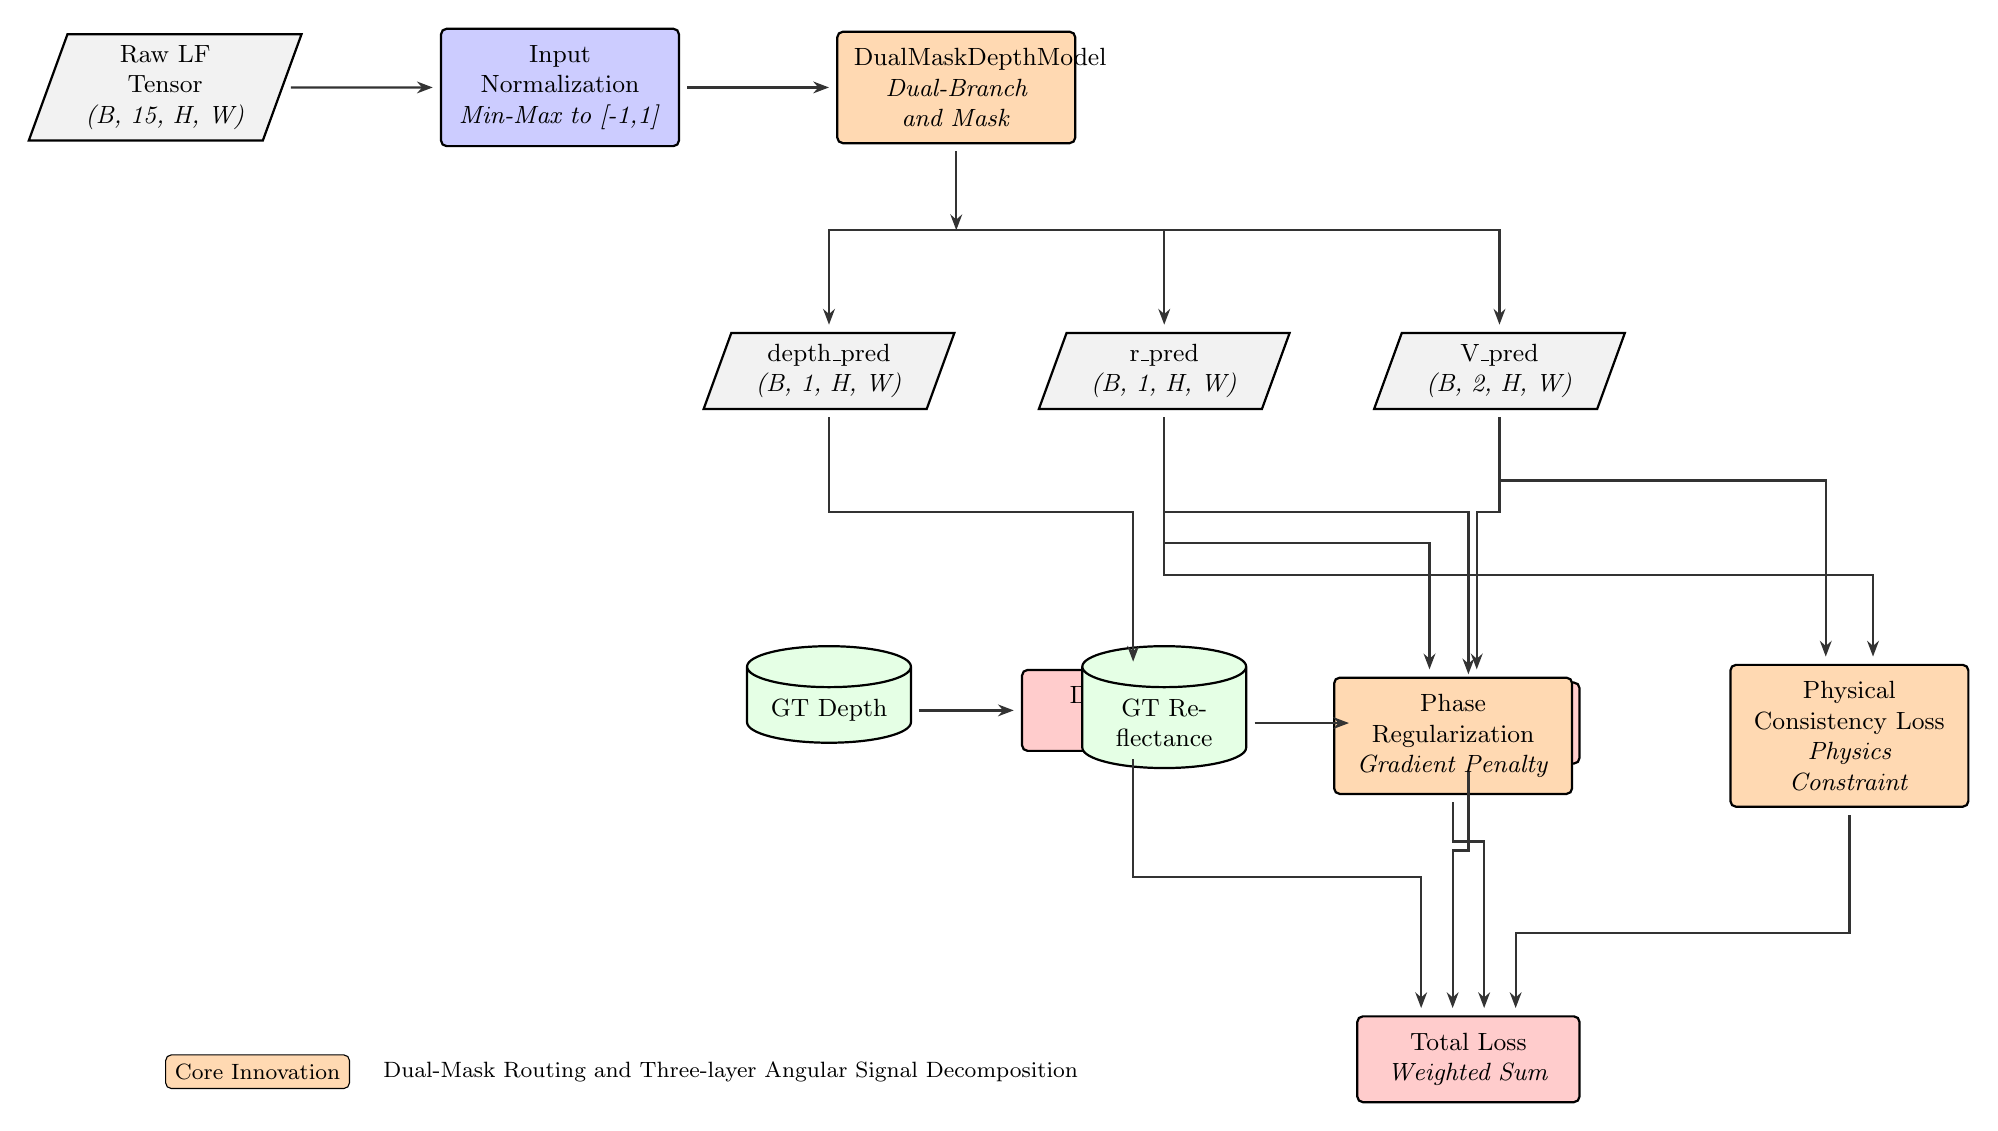
\begin{tikzpicture}[
  data/.style={
    trapezium, trapezium left angle=70, trapezium right angle=110,
    draw, thick, fill=gray!10, 
    text width=2.2cm, align=center, font=\small,
    inner sep=4pt, outer sep=3pt
  },
  module/.style={
    rectangle, rounded corners=2pt,
    draw, thick, 
    text width=2.6cm, align=center, font=\small,
    inner sep=6pt, outer sep=3pt
  },
  loss/.style={
    rectangle, rounded corners=2pt,
    draw, thick, fill=red!20,
    text width=2.4cm, align=center, font=\small,
    inner sep=6pt, outer sep=3pt
  },
  innov/.style={
    fill=orange!30
  },
  encoder/.style={
    fill=blue!20
  },
  gt/.style={
    cylinder, shape border rotate=90, aspect=0.25,
    draw, thick, fill=green!10,
    text width=1.8cm, align=center, font=\small,
    inner sep=4pt, outer sep=3pt
  },
  arr/.style={
    -{Stealth[length=2mm]}, thick, color=black!80
  },
  skip/.style={
    -{Stealth[length=2mm]}, thick, dashed, color=gray
  }
]

% ================= Row 1: Forward Pass =================
\node[data] (RawLF) {Raw LF Tensor\\ \textit{(B, 15, H, W)}};
\node[module, encoder, right=1.8cm of RawLF] (InputNorm) {Input\\Normalization\\ \textit{Min-Max to [-1,1]}};
\node[module, innov, right=1.8cm of InputNorm] (DualMask) {DualMaskDepthModel\\ \textit{Dual-Branch and Mask}};

% ================= Row 2: Outputs =================
\node[data, below=2.2cm of DualMask.south west, anchor=north] (depth_pred) {depth\_pred\\ \textit{(B, 1, H, W)}};
\node[data, right=1.2cm of depth_pred] (r_pred) {r\_pred\\ \textit{(B, 1, H, W)}};
\node[data, right=1.2cm of r_pred] (V_pred) {V\_pred\\ \textit{(B, 2, H, W)}};

% ================= Row 3: Ground Truth & Basic Losses =================
\node[gt, below=2.8cm of depth_pred] (GT_Depth) {GT Depth};
\node[loss, right=1.2cm of GT_Depth] (DepthLoss) {Depth Loss\\ \textit{MSE}};

\node[gt, below=2.8cm of r_pred] (GT_r) {GT Reflectance};
\node[loss, right=1.2cm of GT_r] (rLoss) {Reflectance Loss\\ \textit{MSE}};

% ================= Row 4: Regularizations =================
\node[module, innov, below=3.2cm of V_pred.south west, anchor=north] (PhaseReg) {Phase\\Regularization\\ \textit{Gradient Penalty}};
\node[module, innov, right=1.8cm of PhaseReg] (PhysCons) {Physical\\Consistency Loss\\ \textit{Physics Constraint}};

% ================= Row 5: Total Loss =================
\node[loss, below=3.0cm of rLoss] (TotalLoss) {Total Loss\\ \textit{Weighted Sum}};

% ================= Connections: Forward Pass =================
\draw[arr] (RawLF) -- (InputNorm);
\draw[arr] (InputNorm) -- (DualMask);

\coordinate (split1) at ([yshift=-1.0cm]DualMask.south);
\draw[arr] (DualMask.south) -- (split1);
\draw[arr] (split1) -| (depth_pred.north);
\draw[arr] (split1) -| (r_pred.north);
\draw[arr] (split1) -| (V_pred.north);

% ================= Connections: Basic Losses =================
\draw[arr] (depth_pred.south) -- ++(0,-1.2) -| (DepthLoss.north);
\draw[arr] (GT_Depth.east) -- (DepthLoss.west);

\draw[arr] (r_pred.south) -- ++(0,-1.2) -| (rLoss.north);
\draw[arr] (GT_r.east) -- (rLoss.west);

% ================= Connections: Regularizations =================
\draw[arr] (V_pred.south) -- ++(0,-1.2) -| ([xshift=0.3cm]PhaseReg.north);
\draw[arr] (r_pred.south) -- ++(0,-1.6) -| ([xshift=-0.3cm]PhaseReg.north);

\draw[arr] (V_pred.south) -- ++(0,-0.8) -| ([xshift=-0.3cm]PhysCons.north);
\draw[arr] (r_pred.south) -- ++(0,-2.0) -| ([xshift=0.3cm]PhysCons.north);

% ================= Connections: Total Loss =================
\draw[arr] (DepthLoss.south) -- ++(0,-1.5) -| ([xshift=-0.6cm]TotalLoss.north);
\draw[arr] (rLoss.south) -- ++(0,-1.0) -| ([xshift=-0.2cm]TotalLoss.north);
\draw[arr] (PhaseReg.south) -- ++(0,-0.5) -| ([xshift=0.2cm]TotalLoss.north);
\draw[arr] (PhysCons.south) -- ++(0,-1.5) -| ([xshift=0.6cm]TotalLoss.north);

% ================= Legend =================
\begin{scope}[shift={(0,-12.5)}]
  \node[draw, rounded corners=2pt, fill=orange!30, font=\footnotesize, anchor=west] (leg1) at (0,0) {Core Innovation};
  \node[font=\footnotesize, anchor=west, right=0.3cm of leg1] {Dual-Mask Routing and Three-layer Angular Signal Decomposition};
\end{scope}

\end{tikzpicture}